\documentclass[12pt]{article}
\usepackage{../mcm}
\graphicspath{{../images/}}

\begin{document}

\section{Shapes}
\subsection{Assumptions on Shapes}
\begin{enumerate}
  \item The area is fixed to $A$. To determine the optimal shape, we use $A=1$. The effects of varying $A$ is explored separately.
\end{enumerate}

\subsection{Mutation, Area-Preserving Map, and Chaos}
In GA, mutation serves as a means of introducing new kinds of shapes that are potentially successful.
Since our goal is to compare different shapes with fixed area, we need to mutate shapes in a way such that does not alter the area.
Thus, mutation of shapes naturally require \textit{area-preserving map}.
Area-preserving map is a measure-preserving map in a two-dimensional sense, i.e. $m(L^{-1}) = m(L)$, where $m$ is the Lebesgue measure.
For example, suppose $L$ is a linear transformation.
If $\det(L) = 1$ then it is an area-preserving map; the class of such maps correspond to the special linear group $SP(2,R)$.
A typical member of $SP(2,R)$, however, does not bring about a radical change to a shape.
For example, the matrix
\begin{equation*}
\begin{pmatrix}
    \cos\theta & -\sin\theta  \\
    \sin\theta & \cos\theta  
  \end{pmatrix}
\end{equation*}
as a linear map corresponds to the rotation by $\theta$. 
Although this characteristic is suitable as a way of introducing slight modifications to a pre-existing shape, applications of such maps would not create an entirely new shape.
The observation motivates us to employ chaotic maps instead.
We can think of chaotic maps as having a higher mutation rate than non-chaotic maps.
Hence, we can use chaotic maps as a way of creating a random shape, which would correspond to generating a random rational number in a usual GA.
Mutations of shapes by area-preserving chaotic maps allow our GA to explore the solution space that would not be easily accessible by non-chaotic transformations.
In particular, we employ two chaotic maps: the \textbf{cat map} and \textbf{kick map}.

\subsection{The Cat Map}
We use the cat map (commonly refered to as the "Arnold's Cat Map") to mutate shapes.
Arnold's cat map is a chaotic, area-preserving map on a two-dimensional torus \citep{hilborn}.
The cat map $F$is defined as
\begin{equation*}
  F: (x,y) \mapsto (2x + y, x + y) \mbox{ (mod 1)}.
\end{equation*}
The corresponding matrix is
\begin{equation*}
A =
\begin{pmatrix}
    2 & 1  \\
    1 & 1  
  \end{pmatrix},
\end{equation*}
and clearly, $\det(A) = 1$.
In order to obtain a wider variety of shapes, we parametrize the Arnold's map as follows:
\begin{equation*}
  F: (x,y) \mapsto (kx + (k-1)y, x + y) \mbox{ (mod 1)},
\end{equation*}
where $k \in \mathbb{R}$, $0 \leq k \leq 5$.
Note that the determinant of the corresponding matrix
\begin{equation*}
\begin{pmatrix}
    k & k-1  \\
    1 & 1  
  \end{pmatrix}
\end{equation*}
is one.
Therefore, the parametrized Arnold's map is area-preserving.
\begin{figure}[t]
  \centering
  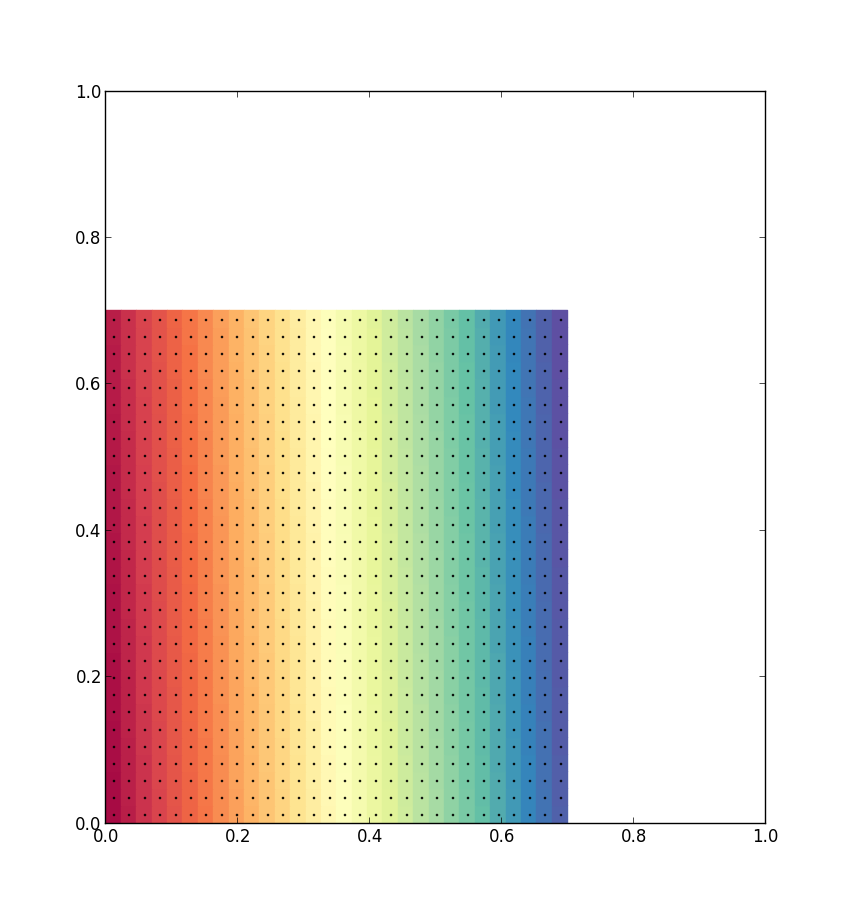
\includegraphics[width=0.6\textwidth]{square_049_900}
  \caption{A square $A = 0.49$ (i.e. the length of each edge is 0.7). Each square consists of patches. This square, for instance, consists of 400 patches, each represented with different colors.}
  \label{fig:square}
\end{figure}
The cat map stretches and folds the domain, and as a result, it produces thin strips.
The parameter $k$ determines the thickness of the strips.
The higher the value of $k$, the thinner the strips are (Fig.~\ref{fig:catmap_demo1}).
\begin{figure}[t]
  \centering
  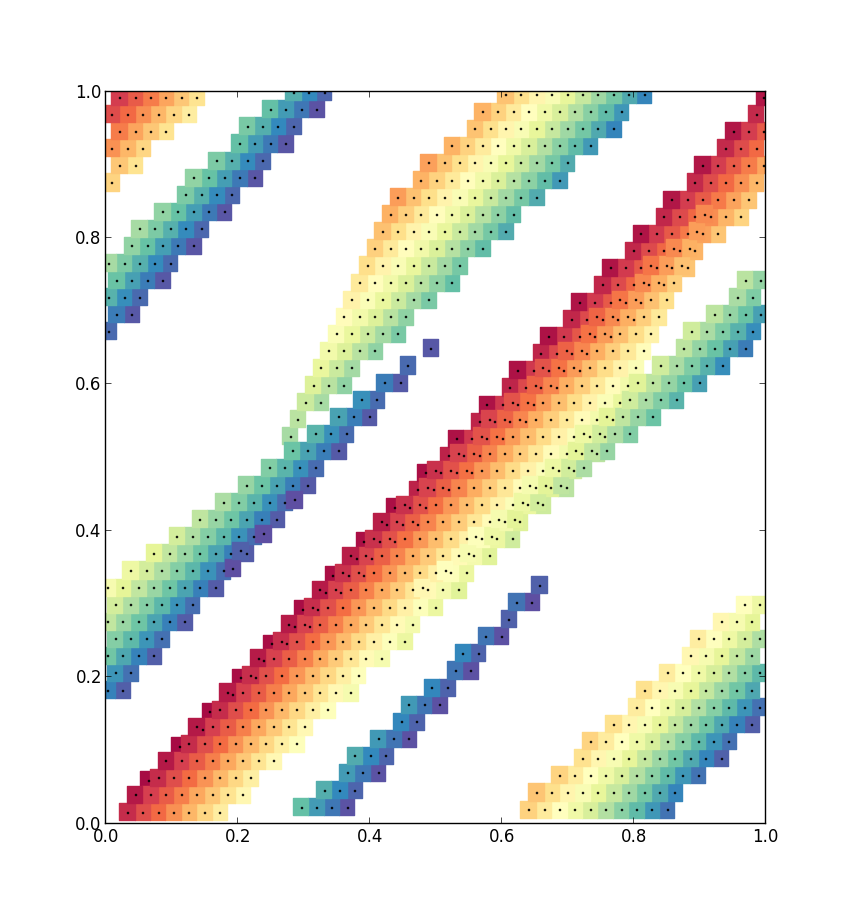
\includegraphics[width=0.4\textwidth]{catmap_1-5}
  \hspace{2cm}
  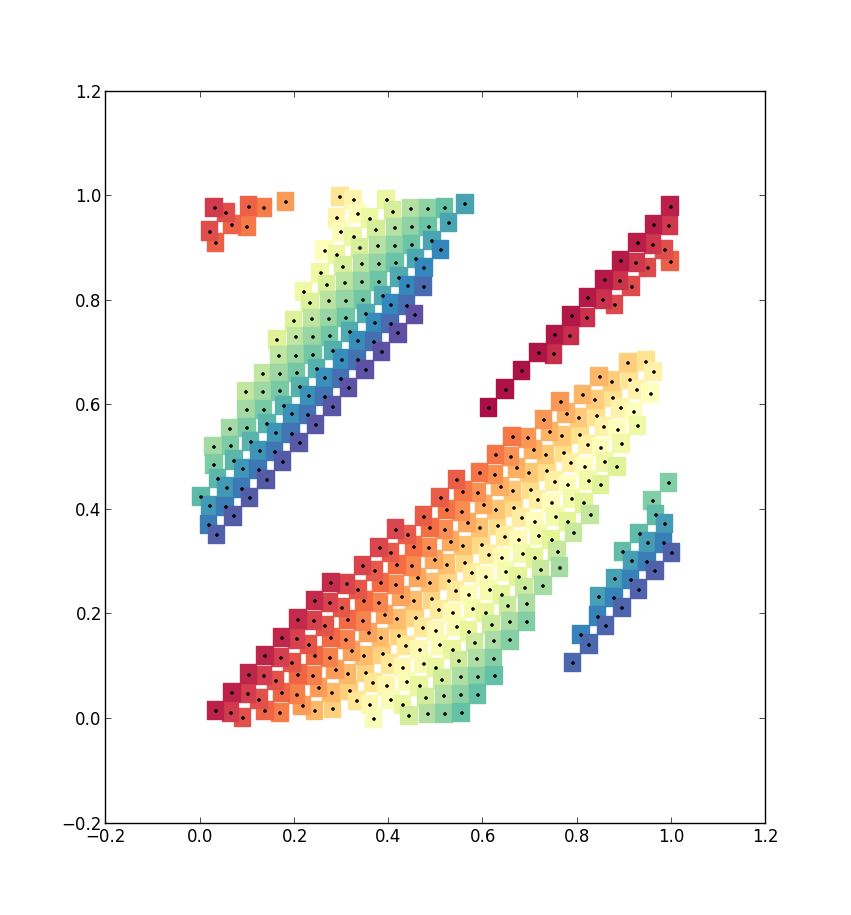
\includegraphics[width=0.4\textwidth]{catmap_3}
  \caption{Cat Map. left: $k=1.5$; right: $k = 3$. After one iteration. 
    Colors of the patches correspond to those in (Fig.~\ref{fig:square}).
    The one with greater $k$ tends to stretch the square to the $x$-direction, and splits the square region into thinner strips.
  }
  \label{fig:catmap_demo1}
\end{figure}

Although, $k$ can be any real number, parameters $k_0$ and its negative $-k_0$ result in effectively the same transformation, since the mapped images would be symmetric about the origin, and we take modulus 1 of the points.
Thus, we can only use $k \in \mathbb{R}^+$ without losing shapes in the solution space.
Also, the cat map would tend to stretch the unit square to the $x$-direction for greater $k$.
We will use $k \leq 10$, because, in a simulation using a limited precision, $k\geq 10$ does not give rise to appreciably different shapes (Fig.~\ref{fig:catmap_demo2}).

\begin{figure}[t]
  \centering
  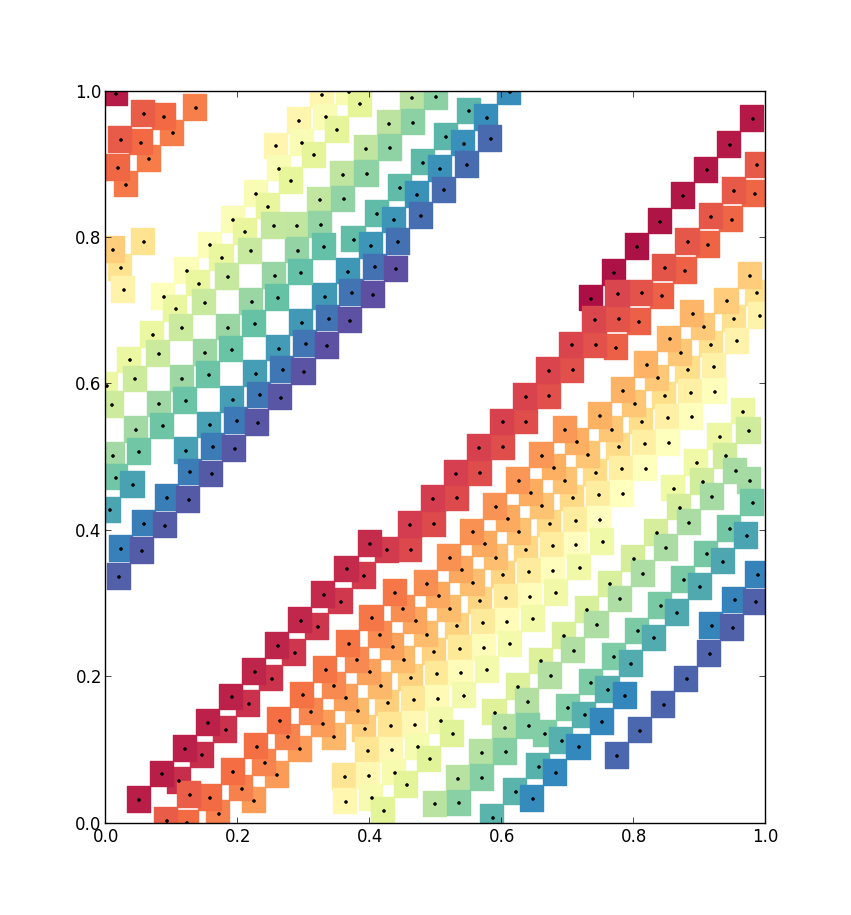
\includegraphics[width=0.4\textwidth]{catmap_10}
  \hspace{2cm}
  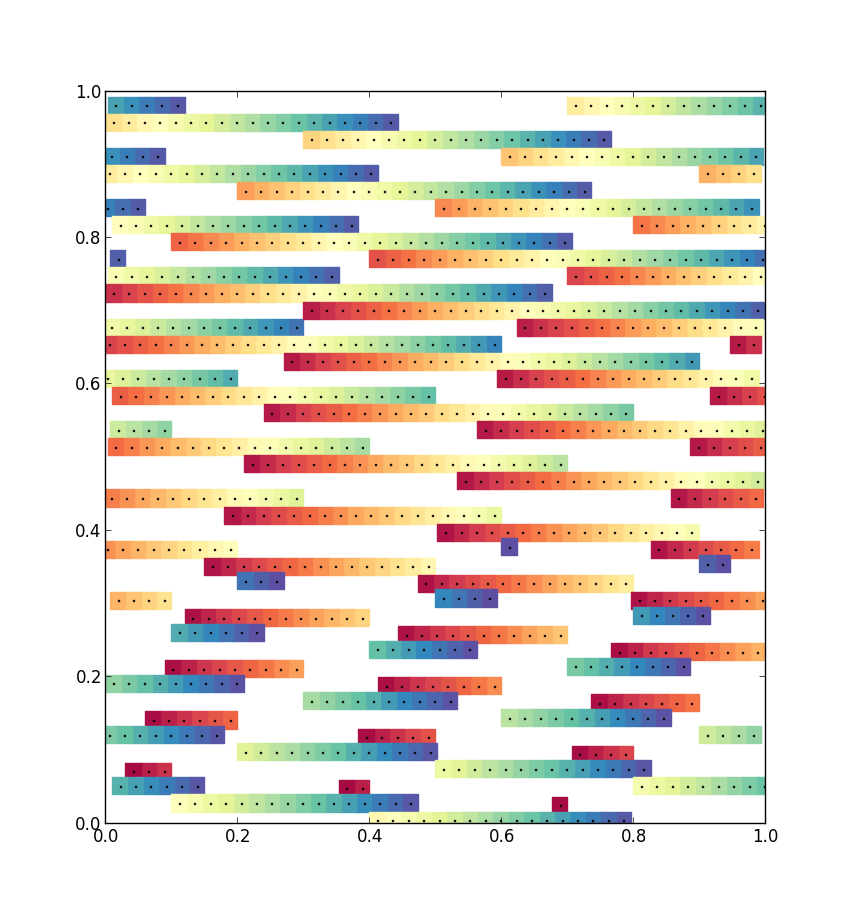
\includegraphics[width=0.4\textwidth]{catmap_30}
  \caption{Cat Map. left: $k=10$; right: $k = 30$. After one iteration. 
    Although the two images are not exactly the same, the differences seem not to be significant from a qualitative point of view.
  }
  \label{fig:catmap_demo2}
\end{figure}

\subsection{The Kick Map}
The other area-preserving chaotic map that we employ, the \textit{kick map}, is usually called the Chirikov's Standard Map \citep{ott}.
Qualitatively, the kick map \textit{swirls} a shape, a complementary action of the cat map, which stretches a shape into thin strips.
The kick map is defined as:
\begin{align*}
  y &\mapsto y + k \sin x \mbox{ (mod $2\pi$)} \\
  x &\mapsto x + y \mbox{ (mod $2\pi$)},
\end{align*}
where updates of $y$ and $x$ are done asyncronously ($y$ first).
The effects of the cat map is stronger for higher value of $k$ (Fig.~\ref{fig:kickmap_demo1}).
%
\begin{figure}[t]
  \centering
  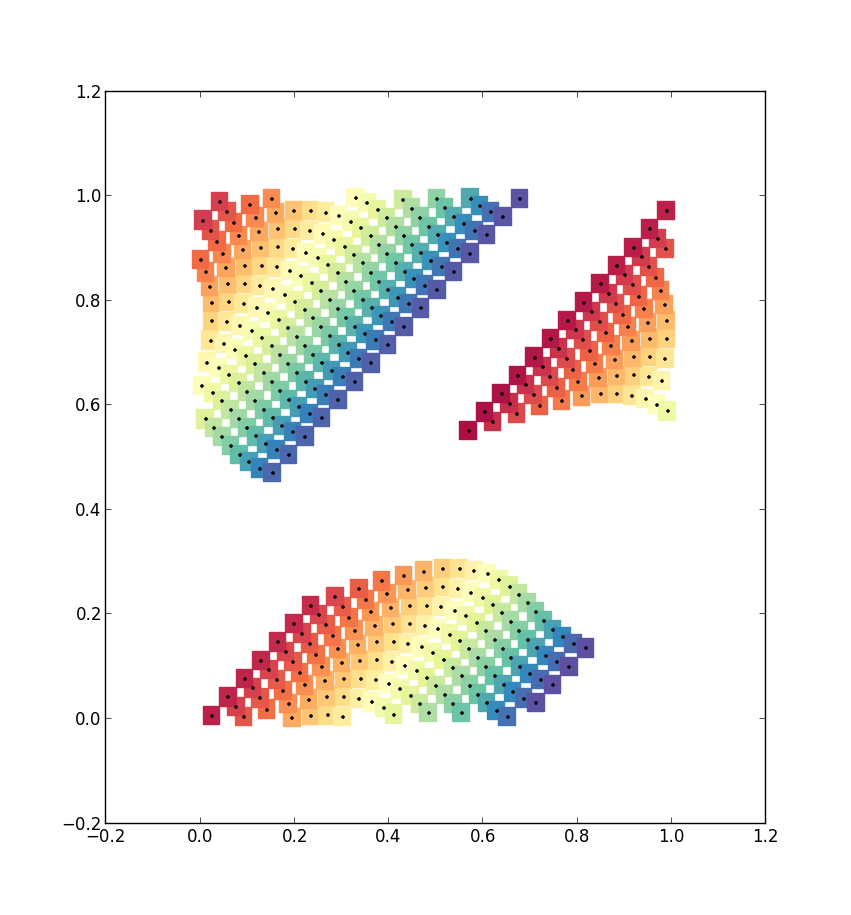
\includegraphics[width=0.4\textwidth]{kickmap_05}
  \hspace{2cm}
  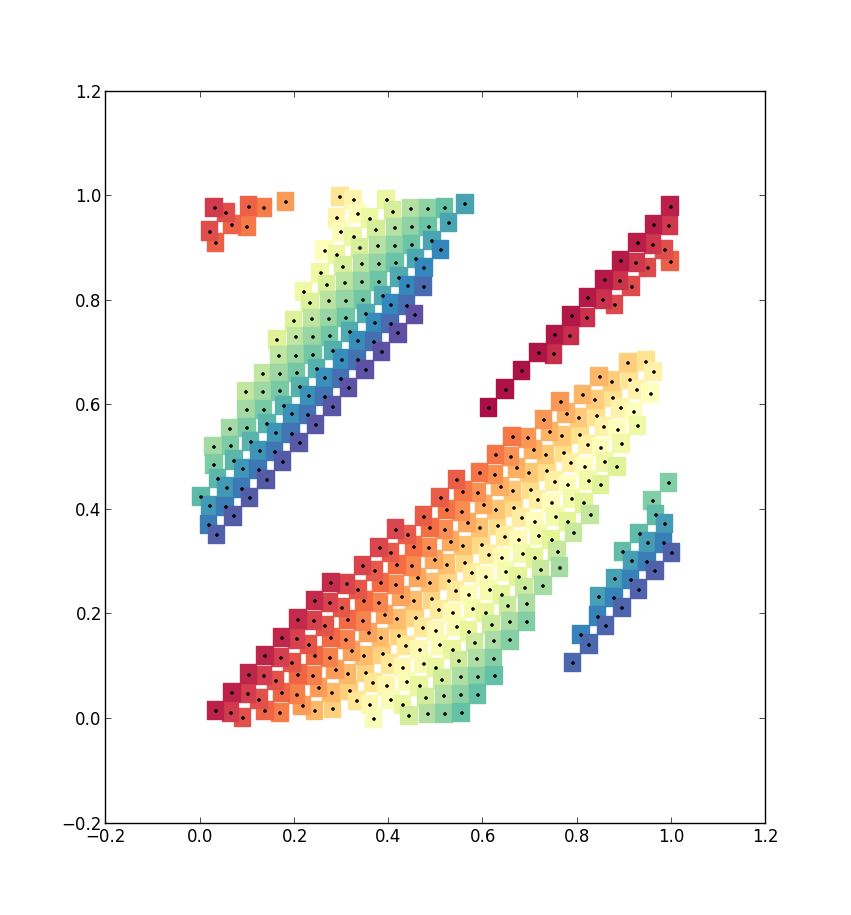
\includegraphics[width=0.4\textwidth]{kickmap_3}
  \caption{The kick map. left: $k=0.5$; right: $k = 3$. After one iteration. 
    The kick map with a higher value of $k$ has stronger effects on the domain.
  }
  \label{fig:kickmap_demo1}
\end{figure}
%
As $k$ approaches $1$, the kick map becomes more and more chaotic.
It is known that the chaotic border is 0.971635... \citep{spedia}.

\begin{figure}[t]
  \centering
  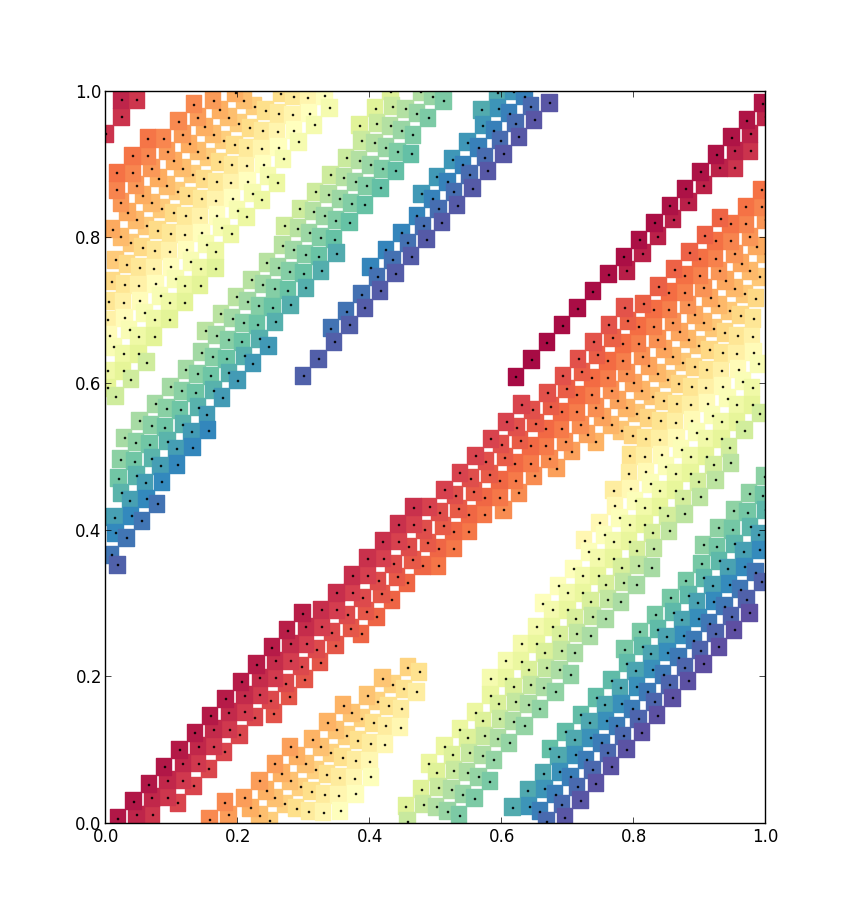
\includegraphics[width=0.4\textwidth]{kickmap_2pi}
  \hspace{2cm}
  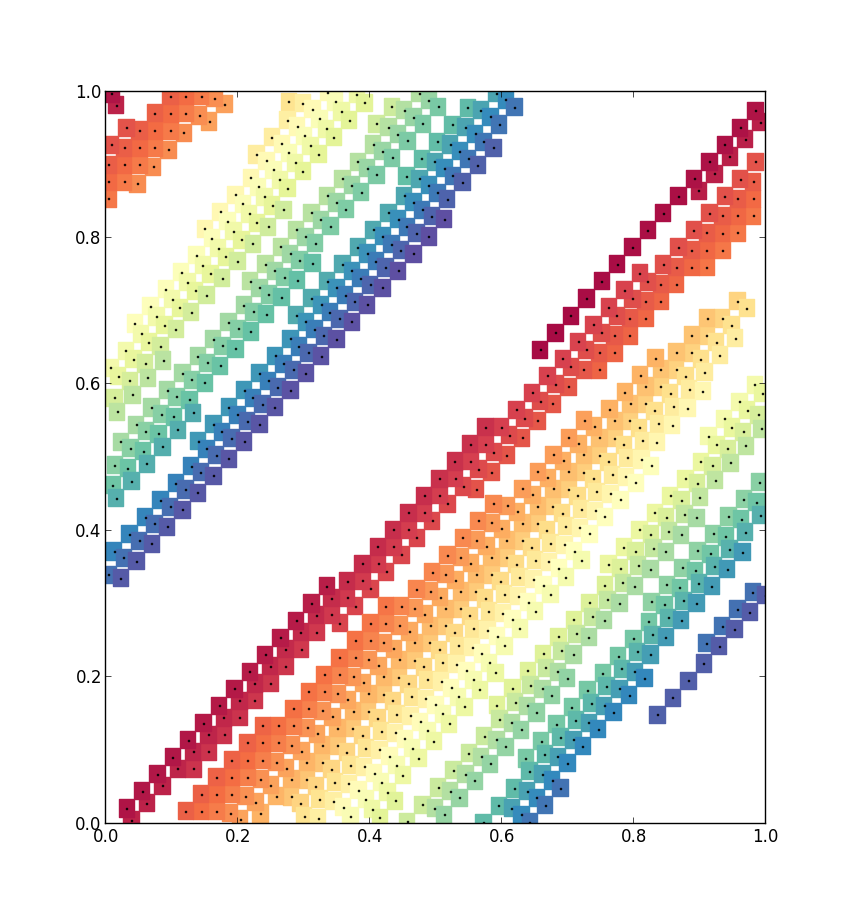
\includegraphics[width=0.4\textwidth]{kickmap_3pi}
  \caption{The kick map. left: $k=10$; right: $k = 30$. After one iteration. 
    Although the two images are not exactly the same, the differences seem not to be significant.
  }
  \label{fig:kickmap_demo2}
\end{figure}

Although we would like to apply the kick map to the unit square, the original kick map is a function from $[0,2\pi] \times [0,2\pi]$ to the same region.
We use the following version of the kick map whose domain and image are the unit square:
\begin{align*}
  y &\mapsto \frac{\pi + 2\pi y + k \sin (2\pi x)}{2\pi} \mbox{ (mod 1)}\\
  x &\mapsto \frac{2\pi (x + y)}{2\pi} \mbox{ (mod 1)}.
\end{align*}
In plain words, the coordinates of each point in the unit square is scaled by $2\pi$ prior to the application of the original kick map, then scale the result by $1/2\pi$.
Taking into account of the chaotic border ($k\approx 1$ in the original kick map), we take the range of $k$ to be $(0,2\pi)$.

\end{document}
